% Options for packages loaded elsewhere
\PassOptionsToPackage{unicode}{hyperref}
\PassOptionsToPackage{hyphens}{url}
\PassOptionsToPackage{dvipsnames,svgnames,x11names}{xcolor}
%
\documentclass[
  letterpaper,
  DIV=11,
  numbers=noendperiod]{scrreprt}

\usepackage{amsmath,amssymb}
\usepackage{iftex}
\ifPDFTeX
  \usepackage[T1]{fontenc}
  \usepackage[utf8]{inputenc}
  \usepackage{textcomp} % provide euro and other symbols
\else % if luatex or xetex
  \usepackage{unicode-math}
  \defaultfontfeatures{Scale=MatchLowercase}
  \defaultfontfeatures[\rmfamily]{Ligatures=TeX,Scale=1}
\fi
\usepackage{lmodern}
\ifPDFTeX\else  
    % xetex/luatex font selection
\fi
% Use upquote if available, for straight quotes in verbatim environments
\IfFileExists{upquote.sty}{\usepackage{upquote}}{}
\IfFileExists{microtype.sty}{% use microtype if available
  \usepackage[]{microtype}
  \UseMicrotypeSet[protrusion]{basicmath} % disable protrusion for tt fonts
}{}
\makeatletter
\@ifundefined{KOMAClassName}{% if non-KOMA class
  \IfFileExists{parskip.sty}{%
    \usepackage{parskip}
  }{% else
    \setlength{\parindent}{0pt}
    \setlength{\parskip}{6pt plus 2pt minus 1pt}}
}{% if KOMA class
  \KOMAoptions{parskip=half}}
\makeatother
\usepackage{xcolor}
\setlength{\emergencystretch}{3em} % prevent overfull lines
\setcounter{secnumdepth}{5}
% Make \paragraph and \subparagraph free-standing
\ifx\paragraph\undefined\else
  \let\oldparagraph\paragraph
  \renewcommand{\paragraph}[1]{\oldparagraph{#1}\mbox{}}
\fi
\ifx\subparagraph\undefined\else
  \let\oldsubparagraph\subparagraph
  \renewcommand{\subparagraph}[1]{\oldsubparagraph{#1}\mbox{}}
\fi

\usepackage{color}
\usepackage{fancyvrb}
\newcommand{\VerbBar}{|}
\newcommand{\VERB}{\Verb[commandchars=\\\{\}]}
\DefineVerbatimEnvironment{Highlighting}{Verbatim}{commandchars=\\\{\}}
% Add ',fontsize=\small' for more characters per line
\usepackage{framed}
\definecolor{shadecolor}{RGB}{241,243,245}
\newenvironment{Shaded}{\begin{snugshade}}{\end{snugshade}}
\newcommand{\AlertTok}[1]{\textcolor[rgb]{0.68,0.00,0.00}{#1}}
\newcommand{\AnnotationTok}[1]{\textcolor[rgb]{0.37,0.37,0.37}{#1}}
\newcommand{\AttributeTok}[1]{\textcolor[rgb]{0.40,0.45,0.13}{#1}}
\newcommand{\BaseNTok}[1]{\textcolor[rgb]{0.68,0.00,0.00}{#1}}
\newcommand{\BuiltInTok}[1]{\textcolor[rgb]{0.00,0.23,0.31}{#1}}
\newcommand{\CharTok}[1]{\textcolor[rgb]{0.13,0.47,0.30}{#1}}
\newcommand{\CommentTok}[1]{\textcolor[rgb]{0.37,0.37,0.37}{#1}}
\newcommand{\CommentVarTok}[1]{\textcolor[rgb]{0.37,0.37,0.37}{\textit{#1}}}
\newcommand{\ConstantTok}[1]{\textcolor[rgb]{0.56,0.35,0.01}{#1}}
\newcommand{\ControlFlowTok}[1]{\textcolor[rgb]{0.00,0.23,0.31}{#1}}
\newcommand{\DataTypeTok}[1]{\textcolor[rgb]{0.68,0.00,0.00}{#1}}
\newcommand{\DecValTok}[1]{\textcolor[rgb]{0.68,0.00,0.00}{#1}}
\newcommand{\DocumentationTok}[1]{\textcolor[rgb]{0.37,0.37,0.37}{\textit{#1}}}
\newcommand{\ErrorTok}[1]{\textcolor[rgb]{0.68,0.00,0.00}{#1}}
\newcommand{\ExtensionTok}[1]{\textcolor[rgb]{0.00,0.23,0.31}{#1}}
\newcommand{\FloatTok}[1]{\textcolor[rgb]{0.68,0.00,0.00}{#1}}
\newcommand{\FunctionTok}[1]{\textcolor[rgb]{0.28,0.35,0.67}{#1}}
\newcommand{\ImportTok}[1]{\textcolor[rgb]{0.00,0.46,0.62}{#1}}
\newcommand{\InformationTok}[1]{\textcolor[rgb]{0.37,0.37,0.37}{#1}}
\newcommand{\KeywordTok}[1]{\textcolor[rgb]{0.00,0.23,0.31}{#1}}
\newcommand{\NormalTok}[1]{\textcolor[rgb]{0.00,0.23,0.31}{#1}}
\newcommand{\OperatorTok}[1]{\textcolor[rgb]{0.37,0.37,0.37}{#1}}
\newcommand{\OtherTok}[1]{\textcolor[rgb]{0.00,0.23,0.31}{#1}}
\newcommand{\PreprocessorTok}[1]{\textcolor[rgb]{0.68,0.00,0.00}{#1}}
\newcommand{\RegionMarkerTok}[1]{\textcolor[rgb]{0.00,0.23,0.31}{#1}}
\newcommand{\SpecialCharTok}[1]{\textcolor[rgb]{0.37,0.37,0.37}{#1}}
\newcommand{\SpecialStringTok}[1]{\textcolor[rgb]{0.13,0.47,0.30}{#1}}
\newcommand{\StringTok}[1]{\textcolor[rgb]{0.13,0.47,0.30}{#1}}
\newcommand{\VariableTok}[1]{\textcolor[rgb]{0.07,0.07,0.07}{#1}}
\newcommand{\VerbatimStringTok}[1]{\textcolor[rgb]{0.13,0.47,0.30}{#1}}
\newcommand{\WarningTok}[1]{\textcolor[rgb]{0.37,0.37,0.37}{\textit{#1}}}

\providecommand{\tightlist}{%
  \setlength{\itemsep}{0pt}\setlength{\parskip}{0pt}}\usepackage{longtable,booktabs,array}
\usepackage{calc} % for calculating minipage widths
% Correct order of tables after \paragraph or \subparagraph
\usepackage{etoolbox}
\makeatletter
\patchcmd\longtable{\par}{\if@noskipsec\mbox{}\fi\par}{}{}
\makeatother
% Allow footnotes in longtable head/foot
\IfFileExists{footnotehyper.sty}{\usepackage{footnotehyper}}{\usepackage{footnote}}
\makesavenoteenv{longtable}
\usepackage{graphicx}
\makeatletter
\def\maxwidth{\ifdim\Gin@nat@width>\linewidth\linewidth\else\Gin@nat@width\fi}
\def\maxheight{\ifdim\Gin@nat@height>\textheight\textheight\else\Gin@nat@height\fi}
\makeatother
% Scale images if necessary, so that they will not overflow the page
% margins by default, and it is still possible to overwrite the defaults
% using explicit options in \includegraphics[width, height, ...]{}
\setkeys{Gin}{width=\maxwidth,height=\maxheight,keepaspectratio}
% Set default figure placement to htbp
\makeatletter
\def\fps@figure{htbp}
\makeatother
\newlength{\cslhangindent}
\setlength{\cslhangindent}{1.5em}
\newlength{\csllabelwidth}
\setlength{\csllabelwidth}{3em}
\newlength{\cslentryspacingunit} % times entry-spacing
\setlength{\cslentryspacingunit}{\parskip}
\newenvironment{CSLReferences}[2] % #1 hanging-ident, #2 entry spacing
 {% don't indent paragraphs
  \setlength{\parindent}{0pt}
  % turn on hanging indent if param 1 is 1
  \ifodd #1
  \let\oldpar\par
  \def\par{\hangindent=\cslhangindent\oldpar}
  \fi
  % set entry spacing
  \setlength{\parskip}{#2\cslentryspacingunit}
 }%
 {}
\usepackage{calc}
\newcommand{\CSLBlock}[1]{#1\hfill\break}
\newcommand{\CSLLeftMargin}[1]{\parbox[t]{\csllabelwidth}{#1}}
\newcommand{\CSLRightInline}[1]{\parbox[t]{\linewidth - \csllabelwidth}{#1}\break}
\newcommand{\CSLIndent}[1]{\hspace{\cslhangindent}#1}

\KOMAoption{captions}{tableheading}
\makeatletter
\makeatother
\makeatletter
\@ifpackageloaded{bookmark}{}{\usepackage{bookmark}}
\makeatother
\makeatletter
\@ifpackageloaded{caption}{}{\usepackage{caption}}
\AtBeginDocument{%
\ifdefined\contentsname
  \renewcommand*\contentsname{Table of contents}
\else
  \newcommand\contentsname{Table of contents}
\fi
\ifdefined\listfigurename
  \renewcommand*\listfigurename{List of Figures}
\else
  \newcommand\listfigurename{List of Figures}
\fi
\ifdefined\listtablename
  \renewcommand*\listtablename{List of Tables}
\else
  \newcommand\listtablename{List of Tables}
\fi
\ifdefined\figurename
  \renewcommand*\figurename{Figure}
\else
  \newcommand\figurename{Figure}
\fi
\ifdefined\tablename
  \renewcommand*\tablename{Table}
\else
  \newcommand\tablename{Table}
\fi
}
\@ifpackageloaded{float}{}{\usepackage{float}}
\floatstyle{ruled}
\@ifundefined{c@chapter}{\newfloat{codelisting}{h}{lop}}{\newfloat{codelisting}{h}{lop}[chapter]}
\floatname{codelisting}{Listing}
\newcommand*\listoflistings{\listof{codelisting}{List of Listings}}
\makeatother
\makeatletter
\@ifpackageloaded{caption}{}{\usepackage{caption}}
\@ifpackageloaded{subcaption}{}{\usepackage{subcaption}}
\makeatother
\makeatletter
\@ifpackageloaded{tcolorbox}{}{\usepackage[skins,breakable]{tcolorbox}}
\makeatother
\makeatletter
\@ifundefined{shadecolor}{\definecolor{shadecolor}{rgb}{.97, .97, .97}}
\makeatother
\makeatletter
\makeatother
\makeatletter
\makeatother
\ifLuaTeX
  \usepackage{selnolig}  % disable illegal ligatures
\fi
\IfFileExists{bookmark.sty}{\usepackage{bookmark}}{\usepackage{hyperref}}
\IfFileExists{xurl.sty}{\usepackage{xurl}}{} % add URL line breaks if available
\urlstyle{same} % disable monospaced font for URLs
\hypersetup{
  pdftitle={Introdução à R e Python},
  pdfauthor={Magno Severino},
  colorlinks=true,
  linkcolor={blue},
  filecolor={Maroon},
  citecolor={Blue},
  urlcolor={Blue},
  pdfcreator={LaTeX via pandoc}}

\title{Introdução à R e Python}
\author{Magno Severino}
\date{2026-04-02}

\begin{document}
\maketitle
\ifdefined\Shaded\renewenvironment{Shaded}{\begin{tcolorbox}[breakable, frame hidden, interior hidden, enhanced, borderline west={3pt}{0pt}{shadecolor}, sharp corners, boxrule=0pt]}{\end{tcolorbox}}\fi

\renewcommand*\contentsname{Table of contents}
{
\hypersetup{linkcolor=}
\setcounter{tocdepth}{2}
\tableofcontents
}
\bookmarksetup{startatroot}

\hypertarget{introduuxe7uxe3o}{%
\chapter*{Introdução}\label{introduuxe7uxe3o}}
\addcontentsline{toc}{chapter}{Introdução}

\markboth{Introdução}{Introdução}

Este livro é composto por notas de aula do minicurso de introdução às
linguagens de programação R e Python.

\part{Aprendendo R}

\hypertarget{fundamentos-de-r}{%
\chapter{Fundamentos de R}\label{fundamentos-de-r}}

\hypertarget{rstudio}{%
\section{RStudio}\label{rstudio}}

Para instalação, faça o download do R em \url{http://www.r-project.org}.
Em seguida, instale a IDE (Integrated Development Environment)
\href{http://www.rstudio.org}{R Studio}.

Ao abrir o RStudio, clique no menu \emph{File}/ \emph{New File}/ \emph{R
Script} (ou Ctrl+Shift+N). Você deve ver uma estrutura como a mostrada
na figura abaixo.

\begin{figure}

{\centering 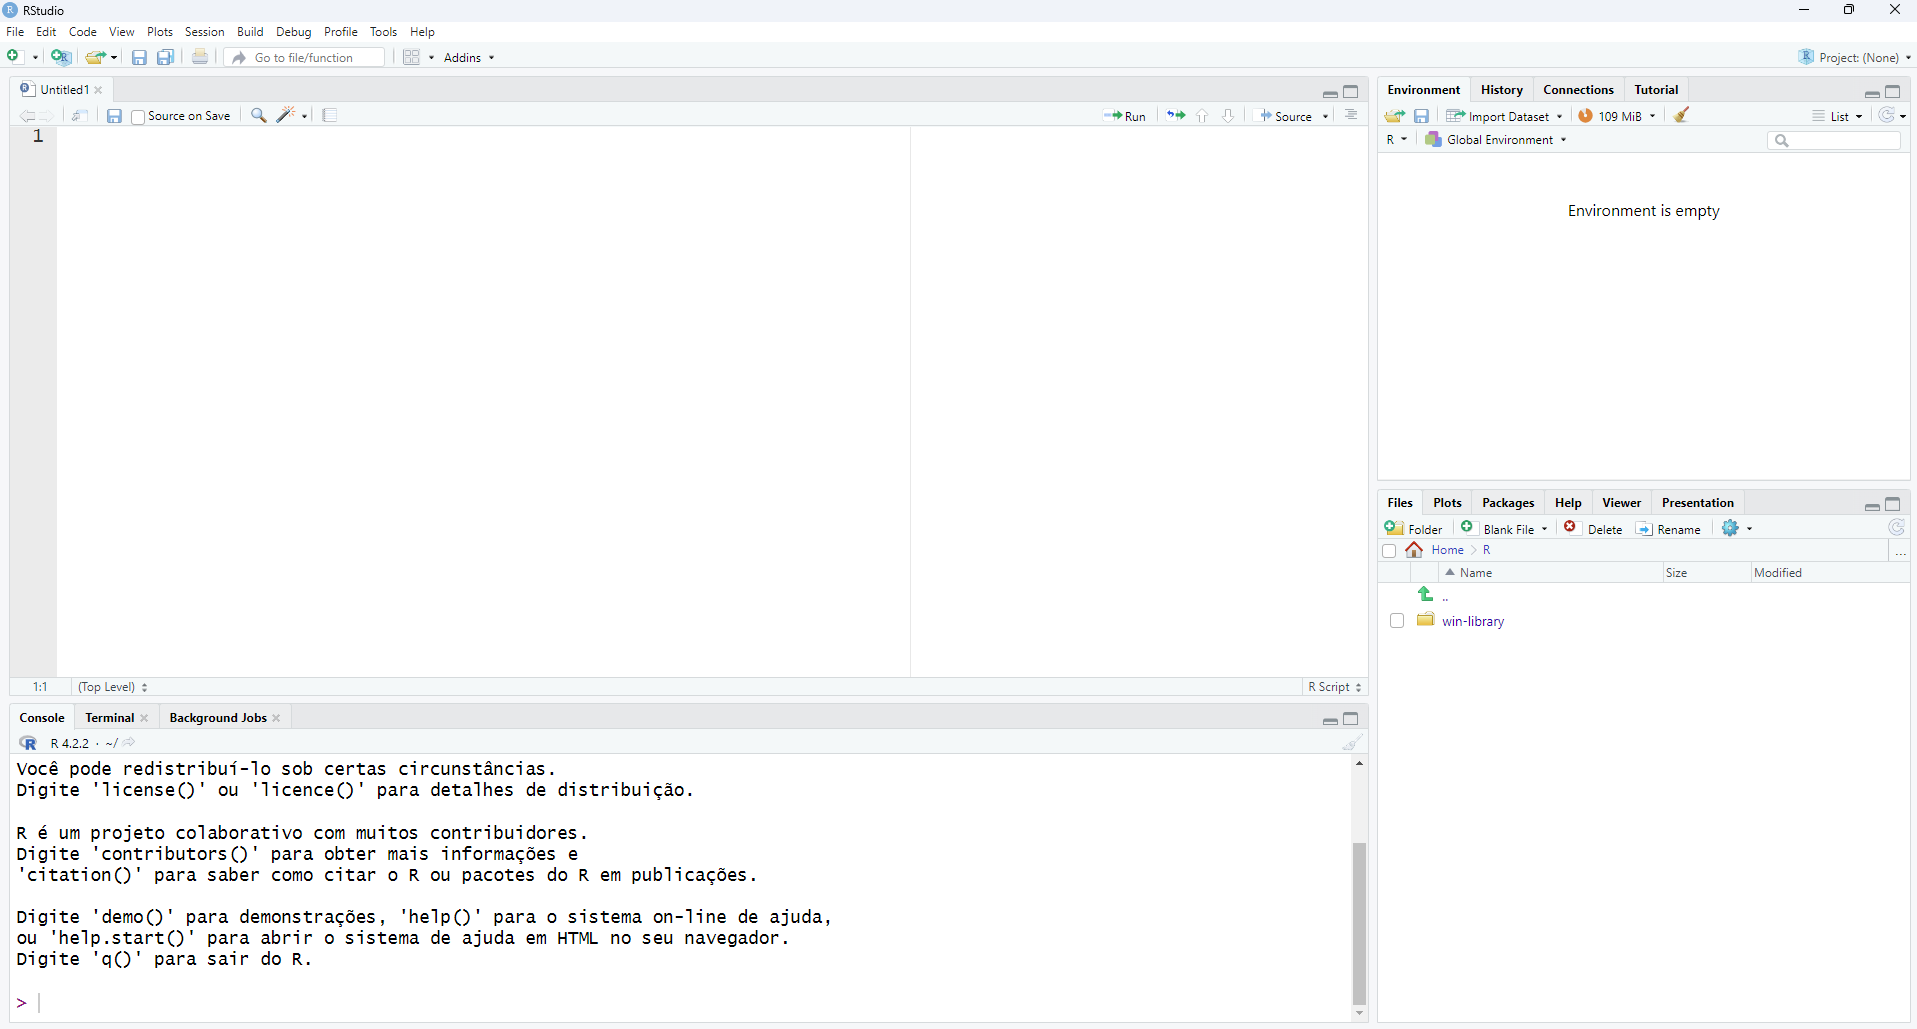
\includegraphics{img/rstudio.png}

}

\caption{Interface do Rstudio}

\end{figure}

Note que são quatro paineis:

\begin{itemize}
\item
  \emph{Painel de Scripts} (superior esquerdo): este painel é onde você
  pode escrever, editar e executar scripts R. Ele fornece recursos como
  destaque de sintaxe, autocompletar e verificação de código para ajudar
  na escrita de código.
\item
  \emph{Painel de Console} (inferior esquerdo):o console é onde o código
  R é executado e os resultados são exibidos. Você pode inserir comandos
  diretamente aqui e ver imediatamente os resultados. Ele também mantém
  um histórico de comandos executados, o que pode ser útil para
  referência futura.
\item
  \emph{Ambiente/Workspace} (superior direito): este painel exibe
  informações sobre os objetos (como variáveis, funções, etc.)
  atualmente carregados na memória do R. Ele mostra detalhes como o nome
  do objeto, tipo de objeto e seu valor atual. Isso é útil para
  monitorar e gerenciar objetos durante uma sessão de trabalho.
\item
  \emph{Arquivos/Plots/Pacotes/Ajuda} (inferior direito): um painel com
  diversas funcionalidades.

  \begin{itemize}
  \item
    Arquivos: Esta guia permite navegar e gerenciar os arquivos do seu
    projeto. Você pode criar, renomear, excluir e organizar arquivos e
    pastas diretamente dentro do RStudio.
  \item
    Gráficos (Plots): Aqui são exibidos os gráficos gerados pelo R.
    Quando você cria um gráfico usando funções de visualização em R, o
    resultado é exibido nesta guia. Isso facilita a análise visual dos
    seus dados e a inspeção dos gráficos durante o processo de criação.
  \item
    Pacotes: Nesta guia, você pode visualizar e gerenciar os pacotes
    instalados no seu ambiente R. Ela exibe uma lista de todos os
    pacotes instalados, juntamente com sua versão e status (carregado ou
    não). Além disso, você pode instalar novos pacotes, atualizar
    pacotes existentes e carregar ou descarregar pacotes conforme
    necessário para o seu trabalho.
  \item
    Ajuda (Help): Esta guia fornece acesso rápido à documentação e às
    informações de ajuda sobre funções, pacotes e outros recursos do R.
    Você pode pesquisar por tópicos específicos e acessar a documentação
    oficial diretamente no RStudio. Isso é útil para obter informações
    sobre a sintaxe de uma função, exemplos de uso e detalhes sobre os
    parâmetros disponíveis.
  \end{itemize}
\end{itemize}

\hypertarget{sec-tipodedados}{%
\section{Tipos de dados}\label{sec-tipodedados}}

Sempre que estiver aprendendo uma nova linguagem, procure primeiro saber
quais são os tipos de dados básicos que podem ser representandos nessa
linguagem.

Em R, são quatro os tipos básicos de dados disponíveis: numéricos,
lógicos, caracteres e fatores.

\hypertarget{sec-tipodedados-num}{%
\subsection{O tipo de dado numérico}\label{sec-tipodedados-num}}

Os dados \emph{numéricos} (numeric) são usados para expressar valores
quantitativos, como preços, taxas e quantidades, sendo representados por
números inteiros ou decimais.

\begin{Shaded}
\begin{Highlighting}[]
\CommentTok{\# Número inteiro representando quantidade de acoes em uma carteira}
\NormalTok{qtd\_acoes }\OtherTok{\textless{}{-}} \DecValTok{100}

\CommentTok{\# Número de ponto flutuante representando a taxa de inflação}
\NormalTok{taxa\_inflacao }\OtherTok{\textless{}{-}} \FloatTok{3.5}

\CommentTok{\# Verificando a classe de taxa\_inflacao}
\FunctionTok{class}\NormalTok{(taxa\_inflacao)}
\end{Highlighting}
\end{Shaded}

\begin{verbatim}
[1] "numeric"
\end{verbatim}

A função \texttt{class()} é usada para determinar a classe de uma
variável. Em outras palavras, ela fornece informações sobre o tipo de
dado que uma variável representa. Nesse caso acima, a variável
\texttt{taxa\_inflacao} é da classe \texttt{numeric}.

\hypertarget{o-tipo-de-dado-luxf3gico}{%
\subsection{O tipo de dado lógico}\label{o-tipo-de-dado-luxf3gico}}

Os dados \emph{lógicos} (logical) são empregados para representar
estados ou condições, como verdadeiro ou falso, sendo úteis em operações
de lógica e comparação.

\begin{Shaded}
\begin{Highlighting}[]
\CommentTok{\# Verificando se a taxa de juros está aumentando}
\NormalTok{taxa\_juros\_aumentando }\OtherTok{\textless{}{-}} \ConstantTok{TRUE}

\CommentTok{\# Verificando se o preço das ações está caindo}
\NormalTok{queda\_preco\_acoes }\OtherTok{\textless{}{-}} \ConstantTok{FALSE}

\CommentTok{\# Verificando a classe de queda\_preco\_acoes}
\FunctionTok{class}\NormalTok{(queda\_preco\_acoes)}
\end{Highlighting}
\end{Shaded}

\begin{verbatim}
[1] "logical"
\end{verbatim}

\hypertarget{o-tipo-de-dado-caractere}{%
\subsection{O tipo de dado caractere}\label{o-tipo-de-dado-caractere}}

Já os dados do tipo \emph{caractere} (character) são utilizados para
representar texto, como nomes de países, empresas ou categorias, sendo
essenciais em análises descritivas e comunicação de resultados.

\begin{Shaded}
\begin{Highlighting}[]
\CommentTok{\# Nome de um país}
\NormalTok{pais }\OtherTok{\textless{}{-}} \StringTok{"Brasil"}

\CommentTok{\# Nome de uma empresa multinacional}
\NormalTok{empresa }\OtherTok{\textless{}{-}} \StringTok{"Petróleo Brasileiro S.A."}

\CommentTok{\# Verificando a classe de pais}
\FunctionTok{class}\NormalTok{(pais)}
\end{Highlighting}
\end{Shaded}

\begin{verbatim}
[1] "character"
\end{verbatim}

\hypertarget{o-tipo-de-dado-fator}{%
\subsection{O tipo de dado fator}\label{o-tipo-de-dado-fator}}

Os \emph{fatores} (factor) são empregados para representar variáveis
categóricas, como classificações, categorias ou grupos, uma forma
eficiente de lidar com dados discretos e qualitativos.

\begin{Shaded}
\begin{Highlighting}[]
\CommentTok{\# Classificação do risco de crédito de uma empresa}
\NormalTok{risco\_credito }\OtherTok{\textless{}{-}} \FunctionTok{factor}\NormalTok{(}\FunctionTok{c}\NormalTok{(}\StringTok{"Baixo"}\NormalTok{, }\StringTok{"Médio"}\NormalTok{, }\StringTok{"Alto"}\NormalTok{, }\StringTok{"Baixo"}\NormalTok{, }\StringTok{"Alto"}\NormalTok{))}

\CommentTok{\# Verificando a classe de risco\_credito}
\FunctionTok{class}\NormalTok{(risco\_credito)}
\end{Highlighting}
\end{Shaded}

\begin{verbatim}
[1] "factor"
\end{verbatim}

A função \texttt{levels()} retorna os níveis (ou categorias) de um
fator. Isso é útil para entender quais são as categorias representadas
pelo fator e para realizar operações de manipulação de dados com base
nessas categorias.

\begin{Shaded}
\begin{Highlighting}[]
\CommentTok{\# Exibindo os níveis de risco de crédito}
\FunctionTok{levels}\NormalTok{(risco\_credito)}
\end{Highlighting}
\end{Shaded}

\begin{verbatim}
[1] "Alto"  "Baixo" "Médio"
\end{verbatim}

\hypertarget{fundamentos-da-linguagem}{%
\section{Fundamentos da linguagem}\label{fundamentos-da-linguagem}}

O ambiente R refere-se ao espaço de trabalho onde todas as variáveis,
funções e objetos criados durante uma sessão R são armazenados e
manipulados. O ambiente inclui tanto os objetos que você criou quanto os
que são carregados automaticamente por meio de pacotes ou outros
mecanismos de importação de dados (mais sobre pacotes a seguir).

Por exemplo, ao usar a função ls() (que lista os nomes dos objetos no
ambiente atual), podemos ver todos os objetos atualmente presentes no
ambiente R.

\begin{Shaded}
\begin{Highlighting}[]
\FunctionTok{ls}\NormalTok{()}
\end{Highlighting}
\end{Shaded}

Se você executou corretamente todos os comandos da Seção
Section~\ref{sec-tipodedados}, deve obter como resultado no console o
seguinte:

\texttt{{[}1{]}\ "empresa"\ \ \ \ \ \ \ \ \ \ \ \ \ \ \ "pais"\ \ \ \ \ \ \ \ \ \ \ \ \ \ \ \ \ \ "qtd\_acoes"}\strut \\
\texttt{{[}4{]}\ "queda\_preco\_acoes"\ \ \ \ \ "taxa\_inflacao"\ \ \ \ \ \ \ \ \ "taxa\_juros\_aumentando"}

usando R como calculadora numeros especiais

\hypertarget{variuxe1veis}{%
\section{Variáveis}\label{variuxe1veis}}

Na Section~\ref{sec-tipodedados} algumas variáveis foram criadas. Por
exemplo a variável \texttt{empresa} que armazena uma cadeia de
caracteres. Você viu, anteriormente a maneira de listar todas as
variáveis definidas no seu ambiente. Mas, afinal, o que são variáveis?

No R, variáveis são elementos fundamentais usados para armazenar e
manipular dados. Elas são como recipientes que guardam valores, objetos
ou expressões. Quando você atribui um valor a uma variável, está
basicamente dando um nome a esse valor para poder acessá-lo e
manipulá-lo posteriormente.

Por exemplo, ao escrever \texttt{preco\_acao\ \textless{}-\ 10}, você
está criando uma variável chamada \texttt{preco\_acao} e atribuindo a
ela o valor 10. Agora, sempre que você usar \texttt{preco\_acao} em seu
código, estará se referindo a esse valor.

Uma prática comum escolher nomes descritivos para variáveis que ajudem a
entender seu propósito ou conteúdo. Por exemplo, em um contexto
econômico, você pode usar \texttt{preco\_acao} para representar o preço
de uma ação ou \texttt{taxa\_inflacao} para representar a taxa de
inflação.

Para atribuir um valor a uma variável, use o operador
\texttt{\textless{}-}. O operador \texttt{=} também pode ser usado para
atribuir valores a variáveis. Ambos os operadores têm o mesmo efeito
prático na atribuição de valores a variáveis em R. A escolha entre eles
geralmente se resume à preferência pessoal e ao estilo de codificação,
embora alguns guias de estilo de código sugiram o uso do
\texttt{\textless{}-}.

\hypertarget{verificando-o-tipo-de-uma-variuxe1vel}{%
\section{Verificando o tipo de uma
variável}\label{verificando-o-tipo-de-uma-variuxe1vel}}

Vamos usar as funções da família \texttt{is.*} para vericar os tipos de
algumas das variáveis que estão no nosso ambiente de trabalho.

\begin{itemize}
\tightlist
\item
  Para a variável \texttt{empresa}:
\end{itemize}

\begin{Shaded}
\begin{Highlighting}[]
\FunctionTok{is.character}\NormalTok{(empresa)}
\end{Highlighting}
\end{Shaded}

Isso retornará \texttt{TRUE} se a variável \texttt{empresa} for do tipo
caractere (character).

\begin{itemize}
\tightlist
\item
  Para a variável \texttt{pais}:
\end{itemize}

\begin{Shaded}
\begin{Highlighting}[]
\FunctionTok{is.character}\NormalTok{(pais)}
\end{Highlighting}
\end{Shaded}

Assim como para a variável \texttt{empresa}, isso retornará
\texttt{TRUE} se a variável \texttt{pais} for do tipo caractere.

\begin{itemize}
\tightlist
\item
  Para a variável \texttt{qtd\_acoes}:
\end{itemize}

\begin{Shaded}
\begin{Highlighting}[]
\FunctionTok{is.numeric}\NormalTok{(qtd\_acoes)}
\end{Highlighting}
\end{Shaded}

Isso retornará \texttt{TRUE} se a variável \texttt{qtd\_acoes} for do
tipo numérico (numeric).

\begin{itemize}
\tightlist
\item
  Para a variável \texttt{queda\_preco\_acoes}:
\end{itemize}

\begin{Shaded}
\begin{Highlighting}[]
\FunctionTok{is.logical}\NormalTok{(queda\_preco\_acoes)}
\end{Highlighting}
\end{Shaded}

Isso retornará \texttt{TRUE} se a variável \texttt{queda\_preco\_acoes}
for do tipo lógico (logical).

\begin{itemize}
\tightlist
\item
  Para a variável \texttt{taxa\_inflacao}:
\end{itemize}

\begin{Shaded}
\begin{Highlighting}[]
\FunctionTok{is.numeric}\NormalTok{(taxa\_inflacao)}
\end{Highlighting}
\end{Shaded}

Assim como para a variável \texttt{qtd\_acoes}, isso retornará
\texttt{TRUE} se a variável \texttt{taxa\_inflacao} for do tipo
numérico.

\begin{itemize}
\tightlist
\item
  Para a variável \texttt{taxa\_juros\_aumentando}:
\end{itemize}

\begin{Shaded}
\begin{Highlighting}[]
\FunctionTok{is.logical}\NormalTok{(taxa\_juros\_aumentando)}
\end{Highlighting}
\end{Shaded}

Isso retornará \texttt{TRUE} se a variável
\texttt{taxa\_juros\_aumentando} for do tipo lógico.

Esses exemplos ilustram como você pode usar as funções \texttt{is.*}
para verificar o tipo de variáveis, ajudando a garantir que você esteja
manipulando os dados corretamente em suas análises.

Outra família de funções importantes é a das funções \texttt{as.*}. Elas
são usadas para converter um objeto de um tipo para outro. Elas permitem
que você altere o tipo de dado de uma variável, o que pode ser útil em
várias situações, como quando você precisa realizar operações
específicas que exigem um determinado tipo de dado ou quando deseja
garantir a consistência dos tipos de dados em seu código.

Algumas das funções \texttt{as.*} mais comuns incluem:

\begin{itemize}
\tightlist
\item
  \texttt{as.character()}: Converte um objeto para o tipo caractere
  (character).
\end{itemize}

\begin{Shaded}
\begin{Highlighting}[]
\NormalTok{numero }\OtherTok{\textless{}{-}} \DecValTok{123}
\NormalTok{numero\_caractere }\OtherTok{\textless{}{-}} \FunctionTok{as.character}\NormalTok{(numero)}
\end{Highlighting}
\end{Shaded}

\begin{itemize}
\tightlist
\item
  \texttt{as.numeric()}: Converte um objeto para o tipo numérico
  (numeric).
\end{itemize}

\begin{Shaded}
\begin{Highlighting}[]
\NormalTok{texto }\OtherTok{\textless{}{-}} \StringTok{"3.14"}
\NormalTok{numero }\OtherTok{\textless{}{-}} \FunctionTok{as.numeric}\NormalTok{(texto)}
\end{Highlighting}
\end{Shaded}

\begin{itemize}
\tightlist
\item
  \texttt{as.logical()}:
\end{itemize}

\begin{Shaded}
\begin{Highlighting}[]
\NormalTok{numero }\OtherTok{\textless{}{-}} \DecValTok{0}
\NormalTok{logico }\OtherTok{\textless{}{-}} \FunctionTok{as.logical}\NormalTok{(numero)}
\end{Highlighting}
\end{Shaded}

Essas funções são úteis para garantir que os tipos de dados estejam
corretos em seu código e para garantir que você possa realizar as
operações desejadas em seus objetos. No entanto, é importante observar
que nem todas as conversões podem ser bem-sucedidas, especialmente
quando há perda de informações (por exemplo, ao converter de caractere
para numérico). Portanto, é sempre uma boa prática verificar se a
conversão foi feita corretamente e se os dados resultantes são os
esperados.

Veja um exemplo de conversão de caractere para numérico com texto não
numérico:

\begin{Shaded}
\begin{Highlighting}[]
\NormalTok{texto }\OtherTok{\textless{}{-}} \StringTok{"abc"}
\NormalTok{numero }\OtherTok{\textless{}{-}} \FunctionTok{as.numeric}\NormalTok{(texto)}
\end{Highlighting}
\end{Shaded}

\begin{verbatim}
Warning: NAs introduzidos por coerção
\end{verbatim}

Neste exemplo, a tentativa de converter o texto ``abc'' para um número
resultará em um valor \texttt{NA} (Not Available), indicando que a
conversão falhou. Veja que a saída do console indica uma mensagem de
\emph{warning}.

\hypertarget{estruturas-de-dados}{%
\section{Estruturas de dados}\label{estruturas-de-dados}}

Em toda análises de dados, é comum lidar com conjuntos de dados que
possuem diferentes estruturas e formatos. Vamos explorar quatro
estruturas de dados fundamentais em R: vetor, matriz, lista e DataFrame.

\hypertarget{vetores}{%
\subsection{Vetores}\label{vetores}}

Um vetor em R é uma estrutura de dados unidimensional que armazena uma
sequência ordenada de elementos do mesmo tipo. A função \texttt{c} nos
ajuda a criar vetores.

\begin{Shaded}
\begin{Highlighting}[]
\CommentTok{\# Vetor de preços de ações}
\NormalTok{precos\_acoes }\OtherTok{\textless{}{-}} \FunctionTok{c}\NormalTok{(}\DecValTok{100}\NormalTok{, }\DecValTok{110}\NormalTok{, }\DecValTok{105}\NormalTok{, }\DecValTok{120}\NormalTok{, }\DecValTok{115}\NormalTok{)}
\end{Highlighting}
\end{Shaded}

Em alguns casos, é de interesse definir sequências de números usando os
operadores \texttt{:} e a função \texttt{seq()}.

\begin{Shaded}
\begin{Highlighting}[]
\CommentTok{\# Vetor de números de 1 a 10}
\NormalTok{sequencia }\OtherTok{\textless{}{-}} \DecValTok{1}\SpecialCharTok{:}\DecValTok{10}
\NormalTok{sequencia}
\end{Highlighting}
\end{Shaded}

\begin{verbatim}
 [1]  1  2  3  4  5  6  7  8  9 10
\end{verbatim}

\begin{Shaded}
\begin{Highlighting}[]
\CommentTok{\# Vetor de números de 1 a 10 com incremento de 2}
\NormalTok{sequencia\_incremento }\OtherTok{\textless{}{-}} \FunctionTok{seq}\NormalTok{(}\AttributeTok{from =} \DecValTok{1}\NormalTok{, }\AttributeTok{to =} \DecValTok{10}\NormalTok{, }\AttributeTok{by =} \DecValTok{2}\NormalTok{)}
\NormalTok{sequencia\_incremento}
\end{Highlighting}
\end{Shaded}

\begin{verbatim}
[1] 1 3 5 7 9
\end{verbatim}

Para verificar o tamanho de um vetor, você pode usar a função
\texttt{length()}.

\begin{Shaded}
\begin{Highlighting}[]
\CommentTok{\# Verificando o tamanho do vetor de preços de ações}
\FunctionTok{length}\NormalTok{(precos\_acoes)}
\end{Highlighting}
\end{Shaded}

\begin{verbatim}
[1] 5
\end{verbatim}

\begin{Shaded}
\begin{Highlighting}[]
\FunctionTok{length}\NormalTok{(}\DecValTok{1}\SpecialCharTok{:}\DecValTok{10}\NormalTok{)}
\end{Highlighting}
\end{Shaded}

\begin{verbatim}
[1] 10
\end{verbatim}

Para acessar elementos em um vetor em R, você pode usar índices
numéricos ou lógicos dentro dos colchetes \texttt{{[}\ {]}}.

Você pode acessar elementos usando índices numéricos dentro dos
colchetes {[} {]}. Por exemplo, \texttt{vetor{[}i{]}} acessa o elemento
na posição \texttt{i} do \texttt{vetor}.

\begin{Shaded}
\begin{Highlighting}[]
\CommentTok{\# Vetor de preços de ações}
\NormalTok{precos\_acoes }\OtherTok{\textless{}{-}} \FunctionTok{c}\NormalTok{(}\DecValTok{100}\NormalTok{, }\DecValTok{110}\NormalTok{, }\DecValTok{105}\NormalTok{, }\DecValTok{120}\NormalTok{, }\DecValTok{115}\NormalTok{)}

\CommentTok{\# Acessando o segundo elemento do vetor}
\NormalTok{segundo\_elemento }\OtherTok{\textless{}{-}}\NormalTok{ precos\_acoes[}\DecValTok{2}\NormalTok{]}

\CommentTok{\# Acessando uma série de elementos do vetor}
\NormalTok{varios\_elementos }\OtherTok{\textless{}{-}}\NormalTok{ precos\_acoes[}\DecValTok{3}\SpecialCharTok{:}\DecValTok{5}\NormalTok{]}
\end{Highlighting}
\end{Shaded}

Você também pode acessar elementos usando índices lógicos dentro dos
colchetes \texttt{{[}\ {]}}. Por exemplo,
\texttt{vetor{[}indices\_logicos{]}} retorna os elementos do vetor onde
os índices lógicos são TRUE.

\begin{Shaded}
\begin{Highlighting}[]
\CommentTok{\# Acessando preços de ações maiores que 110}
\NormalTok{precos\_maior\_que\_110 }\OtherTok{\textless{}{-}}\NormalTok{ precos\_acoes[precos\_acoes }\SpecialCharTok{\textgreater{}} \DecValTok{110}\NormalTok{]}
\end{Highlighting}
\end{Shaded}

\hypertarget{matrizes}{%
\subsection{Matrizes}\label{matrizes}}

Uma matriz em R é uma estrutura de dados bidimensional que consiste em
linhas e colunas de elementos do mesmo tipo. É útil para representar
conjuntos de dados tabulares, como dados de séries temporais ou matrizes
de covariância.

\begin{Shaded}
\begin{Highlighting}[]
\CommentTok{\# Matriz de retornos de ativos}
\NormalTok{retornos\_ativos }\OtherTok{\textless{}{-}} \FunctionTok{matrix}\NormalTok{(}\FunctionTok{c}\NormalTok{(}\FloatTok{0.05}\NormalTok{, }\FloatTok{0.03}\NormalTok{, }\FloatTok{0.02}\NormalTok{, }\FloatTok{0.04}\NormalTok{, }\FloatTok{0.06}\NormalTok{, }\FloatTok{0.03}\NormalTok{), }
                          \AttributeTok{nrow =} \DecValTok{2}\NormalTok{, }\AttributeTok{byrow =} \ConstantTok{TRUE}\NormalTok{)}
\FunctionTok{rownames}\NormalTok{(retornos\_ativos) }\OtherTok{\textless{}{-}} \FunctionTok{c}\NormalTok{(}\StringTok{"Ação 1"}\NormalTok{, }\StringTok{"Ação 2"}\NormalTok{)}
\FunctionTok{colnames}\NormalTok{(retornos\_ativos) }\OtherTok{\textless{}{-}} \FunctionTok{c}\NormalTok{(}\StringTok{"Ano 1"}\NormalTok{, }\StringTok{"Ano 2"}\NormalTok{, }\StringTok{"Ano 3"}\NormalTok{)}
\end{Highlighting}
\end{Shaded}

O código acima cria uma matriz chamada retornos\_ativos que armazena os
retornos de dois ativos ao longo de três anos.

A função \texttt{matrix()} é usada para criar a matriz. O vetor
\texttt{c(0.05,\ 0.03,\ 0.02,\ 0.04,\ 0.06,\ 0.03)} contém os valores
dos retornos dos ativos, fornecidos em ordem de preenchimento de coluna
(de cima para baixo). Os parâmetros \texttt{nrow\ =\ 2} e
\texttt{byrow\ =\ TRUE} indicam que a matriz deve ter 2 linhas (para
representar os dois ativos) e que os valores devem ser preenchidos por
linha (ou seja, primeiro os retornos para o ano 1, depois para o ano 2 e
assim por diante). As funções \texttt{rownames()} e \texttt{colnames()}
são usadas para atribuir nomes às linhas e colunas da matriz,
respectivamente. No caso das linhas, são atribuídos os nomes ``Ação 1''
e ``Ação 2'', representando os dois ativos. Para as colunas, são
atribuídos os nomes ``Ano 1'', ``Ano 2'' e ``Ano 3'', representando os
anos em que os retornos foram registrados.

A função \texttt{class()} retorna a classe do objeto, que neste caso
será ``matrix'', indicando que retornos\_ativos é uma matriz em R.

A função \texttt{dim()} retorna as dimensões da matriz, ou seja, o
número de linhas e colunas.

\begin{Shaded}
\begin{Highlighting}[]
\CommentTok{\# Verificando as dimensões da matriz}
\FunctionTok{dim}\NormalTok{(retornos\_ativos)}
\end{Highlighting}
\end{Shaded}

\begin{verbatim}
[1] 2 3
\end{verbatim}

Neste caso, o resultado será {[}2, 3{]}, indicando que a matriz possui 2
linhas e 3 colunas.

As funções \texttt{nrow()} e \texttt{ncol()} retornam o número de linhas
e colunas da matriz, respectivamente.

\begin{Shaded}
\begin{Highlighting}[]
\FunctionTok{c}\NormalTok{(}\FunctionTok{nrow}\NormalTok{(retornos\_ativos), }\FunctionTok{ncol}\NormalTok{(retornos\_ativos))}
\end{Highlighting}
\end{Shaded}

\begin{verbatim}
[1] 2 3
\end{verbatim}

A função length() retorna o número total de elementos em um objeto. Para
uma matriz, isso retornará o número total de elementos, ou seja, o
produto do número de linhas pelo número de colunas.

\begin{Shaded}
\begin{Highlighting}[]
\FunctionTok{length}\NormalTok{(retornos\_ativos)}
\end{Highlighting}
\end{Shaded}

\begin{verbatim}
[1] 6
\end{verbatim}

Para acessar linhas, colunas e elementos em uma matriz em R, você pode
usar índices numéricos ou nomes (se definidos). Aqui está como fazer:

\begin{itemize}
\tightlist
\item
  Acessando Linhas e Colunas: Você pode acessar linhas e colunas usando
  índices numéricos dentro dos colchetes {[} {]}. Por exemplo,
  matriz{[}i, {]} acessa a linha i e matriz{[}, j{]} acessa a coluna j.
  Para acessar uma célula específica, você usa matriz{[}i, j{]}, onde i
  é o número da linha e j é o número da coluna.
\end{itemize}

\begin{Shaded}
\begin{Highlighting}[]
\CommentTok{\# Acessando a primeira linha da matriz}
\NormalTok{primeira\_linha }\OtherTok{\textless{}{-}}\NormalTok{ retornos\_ativos[}\DecValTok{1}\NormalTok{, ]}

\CommentTok{\# Acessando a segunda coluna da matriz}
\NormalTok{segunda\_coluna }\OtherTok{\textless{}{-}}\NormalTok{ retornos\_ativos[, }\DecValTok{2}\NormalTok{]}

\CommentTok{\# Acessando o elemento na segunda linha e terceira coluna da matriz}
\NormalTok{elemento }\OtherTok{\textless{}{-}}\NormalTok{ retornos\_ativos[}\DecValTok{2}\NormalTok{, }\DecValTok{3}\NormalTok{]}
\end{Highlighting}
\end{Shaded}

\begin{itemize}
\tightlist
\item
  Acessando Linhas e Colunas por Nomes: Se você definiu nomes para as
  linhas e/ou colunas da matriz, você pode acessá-las usando esses
  nomes.
\end{itemize}

\begin{Shaded}
\begin{Highlighting}[]
\CommentTok{\# Acessando a linha chamada "Ação 1"}
\NormalTok{acao1 }\OtherTok{\textless{}{-}}\NormalTok{ retornos\_ativos[}\StringTok{"Ação 1"}\NormalTok{, ]}

\CommentTok{\# Acessando a coluna chamada "Ano 2"}
\NormalTok{ano2 }\OtherTok{\textless{}{-}}\NormalTok{ retornos\_ativos[, }\StringTok{"Ano 2"}\NormalTok{]}

\CommentTok{\# Acessando o elemento na linha "Ação 2" e coluna "Ano 3"}
\NormalTok{elemento2 }\OtherTok{\textless{}{-}}\NormalTok{ retornos\_ativos[}\StringTok{"Ação 2"}\NormalTok{, }\StringTok{"Ano 3"}\NormalTok{]}
\end{Highlighting}
\end{Shaded}

Em R, diferente de outras linguagens de programação, os índices de
linhas e colunas em matrizes (e também em vetores, listas, etc.) começam
em 1 e não em 0. Isso significa que o primeiro elemento de uma matriz
está no índice 1, o segundo no índice 2, e assim por diante

\hypertarget{listas}{%
\subsection{Listas}\label{listas}}

Em R, uma lista é uma estrutura de dados flexível que pode conter
elementos de diferentes tipos, como vetores, matrizes, outras listas e
até mesmo funções. As listas são úteis quando você precisa armazenar e
manipular conjuntos de dados heterogêneos ou estruturas complexas.

Podemos criar uma lista que armazena informações sobre um país, como seu
nome, PIB, taxa de inflação e uma série temporal de valores de câmbio.

\begin{Shaded}
\begin{Highlighting}[]
\CommentTok{\# Criando uma lista com informações sobre um país}
\NormalTok{pais\_info }\OtherTok{\textless{}{-}} \FunctionTok{list}\NormalTok{(}
  \AttributeTok{nome =} \StringTok{"Brasil"}\NormalTok{,}
  \AttributeTok{pib =} \DecValTok{1609}\NormalTok{,}
  \AttributeTok{inflacao =} \FloatTok{0.05}\NormalTok{,}
  \AttributeTok{cambio =} \FunctionTok{c}\NormalTok{(}\FloatTok{4.86}\NormalTok{, }\FloatTok{5.13}\NormalTok{, }\FloatTok{5.20}\NormalTok{, }\FloatTok{5.07}\NormalTok{, }\FloatTok{4.97}\NormalTok{)}
\NormalTok{)}
\end{Highlighting}
\end{Shaded}

Neste exemplo, pais\_info é uma lista que contém quatro elementos:

\begin{itemize}
\tightlist
\item
  \texttt{nome}: o nome do país (tipo caractere).
\item
  \texttt{pib}: o Produto Interno Bruto do país (tipo numérico).
\item
  \texttt{inflacao}: a taxa de inflação do país (tipo numérico).
\item
  \texttt{cambio}: uma série temporal de valores de câmbio do país (tipo
  vetor numérico).
\end{itemize}

Esta lista exemplifica como podemos armazenar diferentes tipos de dados
em uma lista em R. Ela pode ser usada para representar informações
econômicas de um país de forma organizada e acessível.

Para acessar elementos individuais em uma lista pelo nome, usamos o
operador de dólar \texttt{\$}.

\begin{Shaded}
\begin{Highlighting}[]
\CommentTok{\# Acessando o nome do país}
\NormalTok{pais\_info}\SpecialCharTok{$}\NormalTok{nome}
\end{Highlighting}
\end{Shaded}

\begin{verbatim}
[1] "Brasil"
\end{verbatim}

\begin{Shaded}
\begin{Highlighting}[]
\CommentTok{\# Acessando o PIB do país}
\NormalTok{pais\_info}\SpecialCharTok{$}\NormalTok{pib}
\end{Highlighting}
\end{Shaded}

\begin{verbatim}
[1] 1609
\end{verbatim}

Também podemos acessar elementos individuais em uma lista por índice
usando colchetes \texttt{{[}\ {]}}.

\begin{Shaded}
\begin{Highlighting}[]
\CommentTok{\# Acessando o primeiro elemento da lista (nome do país)}
\NormalTok{primeiro\_elemento }\OtherTok{\textless{}{-}}\NormalTok{ pais\_info[[}\DecValTok{1}\NormalTok{]]}

\CommentTok{\# Acessando o terceiro elemento da lista (taxa de inflação)}
\NormalTok{terceiro\_elemento }\OtherTok{\textless{}{-}}\NormalTok{ pais\_info[[}\DecValTok{3}\NormalTok{]]}
\end{Highlighting}
\end{Shaded}

Você deve ter notado o uso de colchetes duplos para acessar os elementos
da lista. Em R, os colchetes simples (\texttt{{[}{]}}) e duplos
(\texttt{{[}{[}{]}{]}}) têm diferentes propósitos quando usados para
acessar elementos em uma lista.

Em resumo, os colchetes simples são usados para acessar subconjuntos de
elementos em uma lista, preservando sua estrutura, enquanto os colchetes
duplos são usados para acessar valores individuais de uma lista, sem
preservar a estrutura original.

\hypertarget{dataframes}{%
\subsection{DataFrames}\label{dataframes}}

vetor, matriz, listas, dataframe

utilizando R como calculadora, números especiais

\hypertarget{exercuxedcios}{%
\section{Exercícios}\label{exercuxedcios}}

utilize a funcao class e avalie a diferenca entre pais\_info{[}1{]} e e
pais\_info{[}{[}2{]}{]}

\hypertarget{fluxos-de-execuuxe7uxe3o}{%
\chapter{Fluxos de execução}\label{fluxos-de-execuuxe7uxe3o}}

\hypertarget{estruturas-condicionais}{%
\section{Estruturas condicionais}\label{estruturas-condicionais}}

if, else,

\hypertarget{estruturas-de-repetiuxe7uxe3o}{%
\section{Estruturas de repetição}\label{estruturas-de-repetiuxe7uxe3o}}

while e for

\hypertarget{manipulauxe7uxe3o-de-dados}{%
\chapter{Manipulação de dados}\label{manipulauxe7uxe3o-de-dados}}

\hypertarget{importar-arquivos-externos}{%
\section{Importar arquivos externos}\label{importar-arquivos-externos}}

\hypertarget{o-pacote-tidyverse}{%
\section{O pacote tidyverse}\label{o-pacote-tidyverse}}

focar no tidyr e no dplyr

\hypertarget{visualizauxe7uxe3o-de-dados}{%
\chapter{Visualização de dados}\label{visualizauxe7uxe3o-de-dados}}

In summary, this book has no content whatsoever.

\begin{Shaded}
\begin{Highlighting}[]
\DecValTok{1} \SpecialCharTok{+} \DecValTok{1}
\end{Highlighting}
\end{Shaded}

\begin{verbatim}
[1] 2
\end{verbatim}

\part{Aprendendo Python}

\hypertarget{fundamentos-de-python}{%
\chapter{Fundamentos de Python}\label{fundamentos-de-python}}

\hypertarget{visualizauxe7uxe3o-de-dados-1}{%
\chapter{Visualização de dados}\label{visualizauxe7uxe3o-de-dados-1}}

\bookmarksetup{startatroot}

\hypertarget{references}{%
\chapter*{References}\label{references}}
\addcontentsline{toc}{chapter}{References}

\markboth{References}{References}

\hypertarget{refs}{}
\begin{CSLReferences}{0}{0}
\end{CSLReferences}



\end{document}
